\subsection{View} \label{subsec:view}
Die View ist als GridBagLayout organisiert und enthält die im Kapitel \ref{subsec:uebersicht} erwähnten Panels.
\bigskip

\paragraph{InputPanel} \label{par:inputpanel}

Das InputPanel hat den Controller und ist im GridBagLayout organisiert. Das Panel wird in mehreren Subpanels unterteilt. Diese sind in der Abbildung  \ref{fig:subpanels} abgebildet. 

\begin{figure}[H]
	\centering
	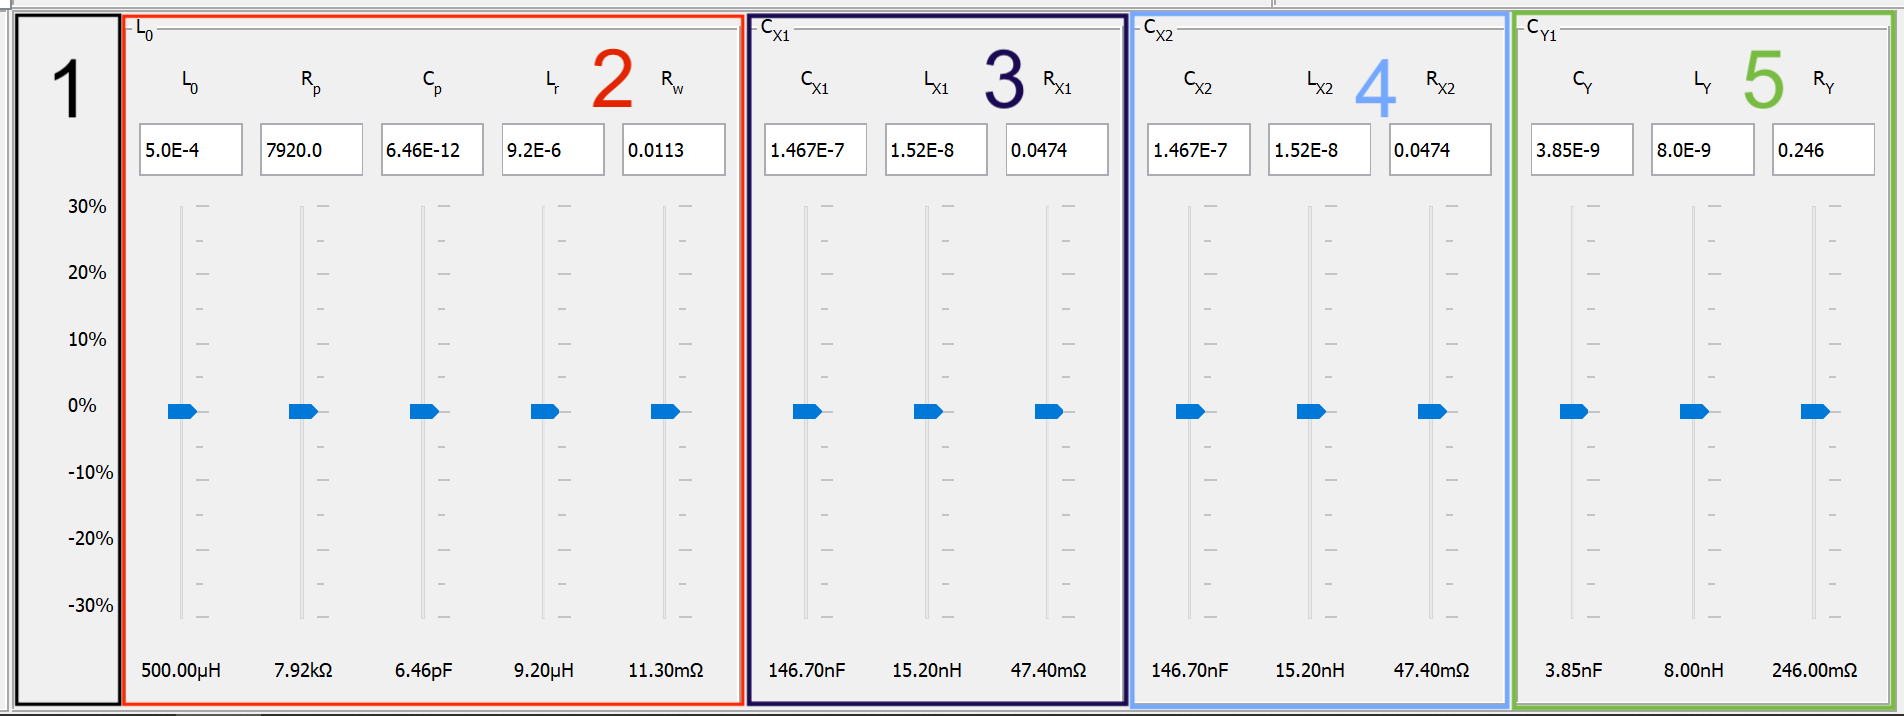
\includegraphics[width=16cm]{SubPanels.png}
	\caption{InputSubPanels}
	\label{fig:subpanels}
\end{figure} 

Das InformationPanel(1) ist im Null-Layout organisiert. Es werden die Prozentzahlen der Schieberegler dargestellt. Diese sind an einer festen Position, da die Grösse des InputPanels nicht verändert werden kann. Die weiteren Subpanels (2-5) sind im GridBagLayout organisiert. In diesen Panels befinden sich die Komponenten der modellierten realen Bauteile. Jede Komponente besitzt ein Textfeld, einen Slider und ein Label. Im Textfeld kann der Benutzer seine Werte für die Komponenten eintragen. Beim Aufstarten des Programmes wird das Feld mit einem Standardwert, der vom Auftragdokument übernommen wurde, geladen. Mit der Klasse JEngineerField werden die Eingaben geprüft. Es ist nur möglich Zahlen einzugeben. Grosse und kleine Zahlen können zur Vereinfachung in wissenschaftlicher Schreibweise (18e-12) oder in Einheiten-Schreibweise (18p) eingetragen werden. Die Ausgabe ist als Einheiten-Schreibweise vordefiniert. Mit dem Schieberegler wird der im Textfeld eingegebene Wert um $\pm$ 30\% verändert und im Label als effektiver Wert ausgegeben. Das Textfeld besitzt einen ActionListener und der Slider einen ChangeListener. Bei einem Ereignis wird die dazugehörige Methode im Controller  aufgerufen.
\bigskip

\paragraph{FiltertablePanel} \label{par:filterpanel}

Das FiltertablePanel hat den Controller und ist im GridBagLayout organisiert. Es enthält eine Tabelle, in der die Parameterwerte hinterlegt und zu dem entsprechenden Filter zugeordnet werden. Jeder Filter in der Tabelle besitzt eine Checkbox, um den Filter zu aktivieren und ein Textfeld, um den Filter  zu benennen. Die Tabelle hat einen TableModelListener und einen ListSelectionListener. Bei einem Ereignis wird die dazugehörige Methode im Controller  aufgerufen.
\bigskip

\newpage

\paragraph{ButtonPanel} \label{par:buttonpanel}

Das ButtonPanel hat den Controller und ist im Null-Layout organisiert. Es enthält die vier Buttons und zwei dazugehörige Labels. Mit diesen kann die Filtertabelle verwaltet und die Speicherverwaltung aufgerufen werden. Jeder Button hat einen ActionListener. Bei einem Ereignis wird die dazugehörige Methode im Controller  aufgerufen.
\bigskip

\paragraph{Plotpanel} \label{par:plotpanel}

Das PlotPanel ist im BorderLayout organisiert. Mit Hilfe des Package JfreeChart \cite{jfreechart} wird die Einfügedämpfung des EMI-Filters in einem Plot dargestellt. Das Package übernimmt viele Funktionen wie das Zoomen des Plots oder das Ändern der Darstellung. Diese Möglichkeiten sind in der Abbildung \ref{fig:einstellung} dargestellt. Löst der Observer ein Ereignis aus, werden die Daten vom Model geholt und geplottet.

\begin{figure}[H]
	\centering
	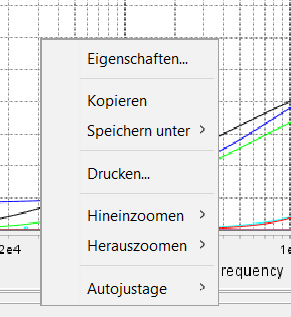
\includegraphics[width=5cm]{Ploteinstellung.png}
	\caption{Einstellungen}
	\label{fig:einstellung}
\end{figure} 

\bigskip
\newpage

\paragraph{Menubar} \label{par:menu}

Das Menubar hat den Controller und ist im Null-Layout organisiert. Es besitzt die Menus File (Abbildung \ref{fig:file}), in dem die Speicherverwaltung aufgerufen werden kann, Circuits (Abbildung \ref{fig:circuits}), in dem die Schaltungen, von denen die Berechnungen ausgehen angezeigt werden und Help (Abbildung \ref{fig:help}), in dem Informationen über das Programm hinterlegt sind. Die Menüs haben einen ActionListener. Bei einem Ereignis wird die dazugehörige Methode im Controller  aufgerufen.

\begin{figure}[H]
	\centering
	\begin{minipage}{0.3\linewidth}
		\centering
		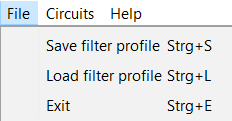
\includegraphics[width=4cm]{file.png}
		\caption{Menupunkt File}
		\label{fig:file}
	\end{minipage}
    %\hfill
    	\begin{minipage}{0.3\linewidth}
	\centering
		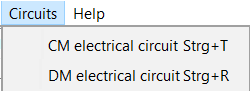
\includegraphics[width=4cm]{circuits.png}
		\caption{Ersatzschaltbilder}
		\label{fig:circuits}
	\end{minipage}
    %\hfill  
        \begin{minipage}{0.3\linewidth}
    \centering
		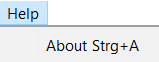
\includegraphics[width=3cm]{help.png}
		\caption{Menupunkt Help}
		\label{fig:help}
    \end{minipage}  
\end{figure}

\newpage

